\chapter{Identificarea bolilor cardiace cu re\c{t}ele neuronale}

\^{I}nainte s\u{a} aplic\u{a}m o re\c{t}ea neuronal\u{a} peste setul nostru de date trebuie mai \^{i}nt\^{a}i s\u{a} le preproces\u{a}m pentru a le converti la un format mai adecvat, s\u{a} elimin\u{a}m unele date nedorite din setul de date care pot \^{i}ngreuna procesul de antrenare \c{s}i s\u{a} ad\u{a}ug\u{a}m unele date care ne vor fi folositoare pe parcurs.

\section{Preprocesarea datelor}

Deoarece datele furnizate de c\u{a}tre The National Heart, Lung, and Blood Institute sunt in format DICOM (Digital Imaging and Communications in Medicine), format destul de greu de lucrat, prima noastr\u{a} sarcin\u{a} va fi s\u{a} le convertim la un format mult mai propice, cum ar fi formatul PNG (Portable Network Graphics), pentru a putea cre\c{s}te viteza de calcul a re\c{t}elei neuronale. \^{I}nainte de a le convertii de la format DICOM la PNG putem s\u{a} mai extragem unele informa\c{t}ii de la fiecare radiografie pe care formatul DICOM le ofer\u{a}, cum ar fi spre exemplu  id-ul pacientului caruia \^{i}i apar\c{t}ine radiografia, numarul de linii \c{s}i de coloane a radiografiei, care definesc marimea , spa\c{t}iul \^{i}ntre pixeli, care reprezint\u{a} o pereche de numere care arat\u{a} distan\c{t}a fizic\u{a} dintre centrii a doi pixeli pe vertical\u{a}, respectiv orizontal\u{a}, acestea fiind m\u{a}surate in milimetrii, ad\^{a}ncimea radiografiei masurat\u{a} in milimetrii, pozi\c{t}ia imaginii, care reprezint\u{a} coordonatele pe axele x, y \c{s}i z, fa\c{t}\u{a} de col\c{t}ul de sus st\^{a}nga al imaginii a centrului  radiografiei facute, loca\c{t}ia relativ\u{a} a radiografiei reprezentat\u{a} in milimetrii \c{s}i axa de codificare a imaginii (dac\u{a} e pe coloan\u{a} sau pe r\^{a}nd ). Toate aceste informa\c{t}ii ne vor fi folositoare pe parcurs a\c{s}a c\u{a} le vom salva \^{i}ntr-un fi\c{s}ier CSV.

\par

Dup\u{a} citirea imaginii vom verifica dac\u{a} imaginea este orientat\u{a} pe coloan\u{a}, \^{i}n acest caz dac\u{a} este adev\u{a}rat  va trebuii s\u{a} calcul\u{a}m transpusa imaginii (liniile vor deveni coloane) \c{s}i s\u{a} o rotim pe orizontal\u{a} de-a lungul axei x, astfel \^{i}nc\^{a}t sus s\u{a} devin\u{a} jos \c{s}i invers, jos s\u{a} devin\u{a} sus, astfel c\u{a} la final imaginea va fi rotit\u{a} cu 90 de grade, iar dintr-o imagine orientat\u{a} pe coloan\u{a} vom avea o imagine orientat\u{a} pe r\^{a}nd. Imediat dup\u{a} aceea va trebuii s\u{a} redimension\u{a}m fiecare imagine, astfel \^{i}nc\^{a}t fiecare s\u{a} aib\u{a} 256 de pixeli \^{i}n \^{i}n\u{a}l\c{t}ime \c{s}i 256 de pixeli \^{i}n l\u{a}\c{t}ime, acest lucru se va face prin decuparea unui patrat de 256 x 256 de pixeli din imaginea original\u{a} care s\u{a} cuprind\u{a} doar inima pacientului, pentru a realiza acest lucru prima dat\u{a} vom verifica dac\u{a} imaginea are dimensiunile mai mici dec\^{a}t dorim noi s\u{a} decup\u{a}m, dac\u{a} da atunci va trebuii s\u{a} adaug\u{a}m un border negru \^{i}n jurul imaginii astfel \^{i}nc\^{a}t s\u{a} ating\u{a} dimensiunea dorit\u{a}. Dup\u{a} ce ne-am asigurat c\u{a} imaginea are o \^{i}n\u{a}l\c{t}ime \c{s}i o l\u{a}\c{t}ime mai mare dec\^{a}t vrem noi s\u{a} decup\u{a}m,  vom calcula punctele de start \c{s}i de final a decup\u{a}rii, astfel \^{i}nc\^{a}t s\u{a} lu\u{a}m fix centrul imaginii, acesta este un compromis destul de bun av\^{a}n \^{i}n vedere faptul c\u{a} fiecare radiografie are inima pacientului situat\u{a} in mijlocul ei.

\par

Acum c\u{a} avem o imagine de dimensiune 256x256 va trebuii s\u{a} aplic\u{a}m metoda CLAHE (Contrast Limited Adaptive Histogram Equalization) pentru a \^{i}mbun\u{a}t\u{a}\c{t}i contrastul \c{s}i calitatea imaginii. CLAHE este o variant\u{a} \^{i}mbunat\u{a}\c{t}it\u{a} a tehnicii de egalizare a histogramei (Histogram Equalization) a unei imagini gri, astfel \^{i}nc\^{a}t histograma aceasteia s\u{a} fie uniform\u{a}, iar fiecare valoare care poate fi \^{i}ntr-o imagine gri, s\u{a} aib\u{a} acela\c{s}i num\u{a}r aproximativ de pixeli. Astfel c\u{a}, fie o imagine f cu $m_r$ linii \c{s}i $m_c$ coloane \c{s}i cu pixeli care au valori \^{i}ntre 0 \c{s}i 255, vom nota cu p ca fiind probabilitatea ca un pixel s\u{a} aib\u{a} valorea n.

$$p_n = \frac{\text{numarul de pixeli cu valoarea n}}{\text{numarul total de pixeli}}$$

Unde n are valori cuprinse intre 0 \c{s}i 255. Atunci metoda de egalizare a histogramei pentru un pixel dintr-o imagine gri, la linia i \c{s}i la coloana c poate fi definit\u{a} \^{i}n felul urm\u{a}tor.

$$g_{i,j} = floor\bigg( 255 \sum_{n=0}^{f{i,j}} p_n \bigg)$$

\^{I}n formula de mai sus, floor face rotunjirea la cel mai apropiat num\u{a}r \^{i}ntreg inferior, iar g reprezint\u{a} noua imagine derivat\u{a} din f, care are histograma pixelilor egalizat\u{a}. Fa\c{t}\u{a} de tehnica de egalizare a histogramei care lucreaz\u{a} pe toat\u{a} imaginea, CLAHE aplic\u{a} acela\c{s}i principiu doar c\u{a} pe un bloc de pixeli, spre exemplu un bloc de pixeli de dimensiune 8x8, dintr-o imagine, acest lucru este necesar pentru a evita schimbarea contrastului \^{i}n regiuni unde acest lucru ar duce la deteliorarea calita\c{t}ii imaginii.

\begin{center}
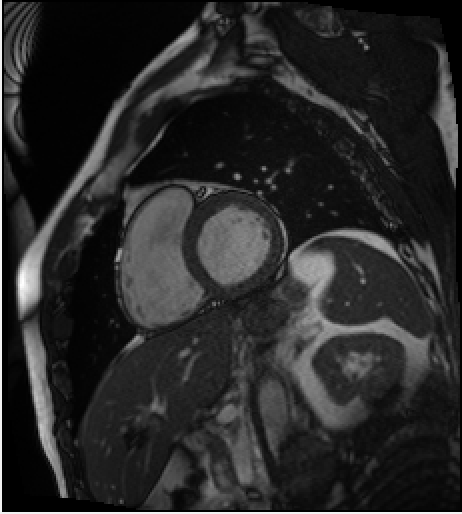
\includegraphics[width=250]{before.png}
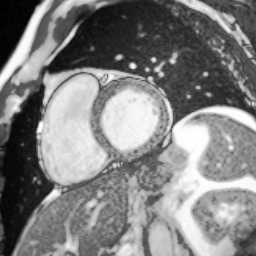
\includegraphics[width=250]{after.png}
\end{center}

Cele dou\u{a} imagini de mai sus reprezint\u{a} un exempu de imagine din setul de date \^{i}nainte de a fi procesat\u{a} \c{s}i dup\u{a} ce a fost procesat\u{a}, cum se poate observa imaginea procesat\u{a} a fost decupat\u{a} din mijlocul imaginii neprocesate, astfel \^{i}nc\^{a}t s\u{a} se elimine o cantitate c\^{a}t mai mare de date care nu sunt necesare pentru scopul nostru, de asemenea se mai poate observa c\u{a} imaginea procesat\u{a} are un contrast mai mare fa\c{t}\u{a} de imaginea neprocesat\u{a}, iar detaliile imaginii se pot observa mai bine, aceste lucruri vor duce la o vitez\u{a} de calcul \c{s}i la o acurate\c{t}e mai mare a re\c{t}elei neuronale.

\par

Cum am precizat mai sus, vom salva intr-un fi\c{s}ier CSV id-ul pacientului, numarul radiografiei, numarul imaginii, numarul de linii \c{s}i de coloane, distan\c{t}a fizic\u{a} \^{i}ntre centrii a doi pixeli, ad\^{a}ncimea radiografiei, locatia radiografiei, planul in care a fost facut\u{a} radiografia ( pe line sau pe coloan\u{a} ) \c{s}i pozi\c{t}ia imaginii fa\c{t}\u{a} de col\c{t}ul din st\^{a}nga sus, pe l\^{a}ng\u{a} toate acestea vom mai salva \c{s}i varianta prin care s-a facut radiografia, c\^{a}nd s-a f\u{a}cut radiografia, firma care a f\u{a}cut aparatul de RMN \c{s}i numele modelului, v\^{a}rsta pacientului, ziua de na\c{s}tere a pacientului, sexul pacientului, numele fi\c{s}ierului \c{s}i orientarea pacientului in imagine. DICOM define\c{s}te un sistem de coordonate numit RCS (Reference Coordinates System) prin care se stabile\c{s}te pozi\c{t}ia corpului  \^{i}n imagine, astfel c\u{a} direc\c{t}ia X este de la m\^{a}na dreapta a pacientului spre m\^{a}na st\^{a}ng\u{a} a acestuia, direc\c{t}ia Y este din fa\c{t}a pacientului spre spatele acestuia, iar direc\c{t}ia Z este de la picioare spre cap, din cauza faptului c\u{a} pozi\c{t}ia corpului este tridimensional\u{a}, iar radiografia este bidimensional\u{a} se va calcula proiec\c{t}ia fiecarei axe definite mai sus la axele unui plan bidimensional, \^{i}n acest caz \^{i}n formatul DICOM se vor gasi \c{s}ase valori care definesc orientarea pacientului in imagine. Primele trei valori reprezint\u{a} proiec\c{t}ia celor trei axe a planului tridimensional la axa X a planului bidimensional (Xx, Xy, Xz), iar celelalte trei valori reprezint\u{a} proiec\c{t}ia celor trei axe a planului tridimensional la axa Y a planului bidimensional (Yx, Yy, Yz), cu aceste valori se poate stabilii foarte u\c{s}or cum este orientat un pacient intr-o radiografie.

\par

Toate valorile salvate mai sus \^{i}n fi\c{s}ierul CSV au fost valori pe care nu am fost nevoi\c{t}i s\u{a} le calcul\u{a}m doarece sunt deja existente \^{i}n fiecare radiografie, \^{i}ns\u{a} pe baza lor putem s\u{a} calcul\u{a}m noi valori care ne vor fi de folos pe parcurs. Una dintre acestea este s\u{a} stabilim timpul dintre dou\u{a} imagini consecutive dintr-o radiografie \c{s}i distan\c{t}a dintre loca\c{t}iile lor, acestea pot fi u\c{s}or calculate prin diferen\c{t}a dintre timpii  celor dou\u{a} imagini \c{s}i a pozi\c{t}iilor pe care le au.

\section{Identificarea ventriculului st\^{a}ng}

Cum se poate observa \c{s}i \^{i}n imaginea de mai jos ventriculul st\^{a}ng este destul de u\c{s}or de identificat cu ochiul liber pentru un om, \^{i}ns\u{a} pentru un calculator aceasta este \^{i}nc\u{a} greu de g\u{a}sit.

\par

Pentru a putea identifica ventriculul st\^{a}ng din astfel de imagine vom avea nevoie de o re\c{t}ea neuronal\u{a} care s\u{a} fac\u{a} segmentarea ventriculului st\^{a}ng de restul de date, iar dup\u{a} aceea se va putea folosii rezultatul ob\c{t}inut pentru calcularea volumului de s\^{a}nge care curge la sistol\u{a} \c{s}i a volumului de s\^{a}nge care curge la diastol\u{a}.

\par

Pentru antrenarea re\c{t}elei neuronale care va face segmentarea inimii vom avea nevoie de un alt set de date, deoarece setul de date pe care \^{i}l avem de la Institutul Na\c{t}ional pentru Inim\u{a}, Pl\u{a}m\^{a}ni \c{s}i S\^{a}nge din America nu ne ofer\u{a} date care s\u{a} indice pozi\c{t}ia exact\u{a} a ventriculului st\^{a}ng \^{i}n radiografie, \^{i}ns\u{a} spitalul Sunnybrook din Canada, Toronto pune la dispozi\c{t}ie date identice care ne ofer\u{a} pozi\c{t}ia exact\u{a} a ventriculului st\^{a}ng \^{i}n radiografie.

\begin{center}
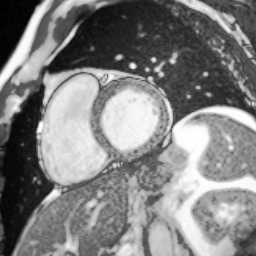
\includegraphics[width=200]{after.png}
\end{center}

\subsection{Datele de la spitalul Sunnybrook}

Cum am precizat \c{s}i mai sus, spitalul Sunnybrook pune la dispozi\c{t}ie un set de date care arat\u{a} pozi\c{t}ia exact\u{a} a ventricului st\^{a}ng a inimii \^{i}n radiografie. Fiecare radiografie a fost f\u{a}cut\u{a} pe parcursul a unui ciclu a inimii, av\^{a}nd o dimensiune de [ 256 x 256 ] de pixeli, iar pentru fiecare radiografie este asociat  un fisier txt cu pozi\c{t}ia exact\u{a} a ventricului st\^{a}ng a inimii.

\begin{center}
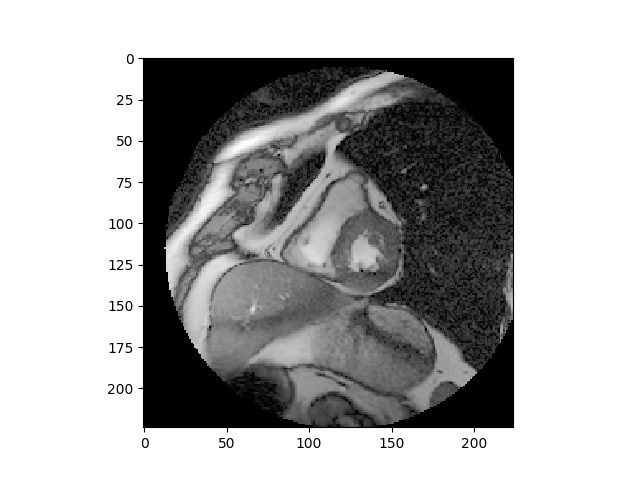
\includegraphics[width=200]{sbh.png}
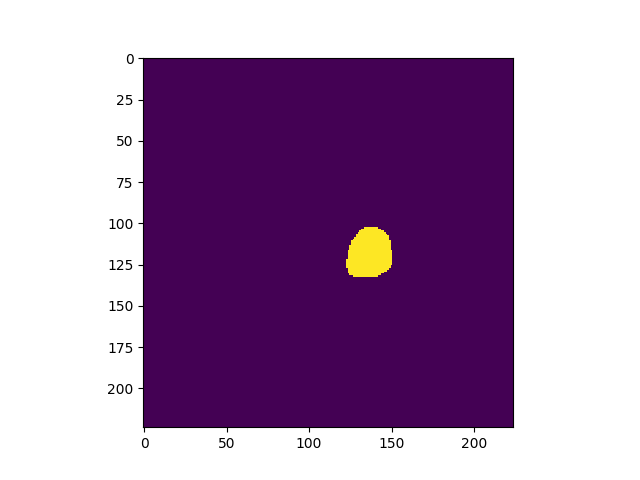
\includegraphics[width=200]{sbl.png}
\end{center}

\^{I}n imaginile de mai sus, avem o radiografie din setul de date Sunnybrook \^{i}n partea din st\^{a}nga, iar \^{i}n partea din dreapta avem pozi\c{t}ia exact\u{a} a ventricului st\^{a}ng \^{i}n radiografie, unde ce este colorat cu mov reprezint\u{a} faptul c\u{a} acolo nu se afl\u{a} ventriculul st\^{a}ng (culoarea mov are asociat\u{a} valoarea 0), iar ce este colorat cu galben reprezint\u{a} faptul c\u{a} acolo se afl\u{a} ventriculul st\^{a}ng (culoarea galben\u{a} are asociat\u{a} valoarea 1). Cu astfel de tipuri de date vom lucra pentru a antrena o re\c{t}ea neuronal\u{a} care s\u{a} fac\u{a} segmentarea ventricului st\^{a}ng a inimii de restul radiografiei. 

\par

La final dup\u{a} ce vom termina s\u{a} antren\u{a}m re\c{t}eaua neuronal\u{a}, vom introduce radiografii de la Institutul Na\c{t}ional pentru Inim\u{a}, Pl\u{a}m\^{a}ni \c{s}i S\^{a}nge din America, ca radiografia de mai sus din st\^{a}nga, iar la final vom ob\c{t}ine pozi\c{t}ia exact\u{a} a ventricului st\^{a}ng, ca \^{i}n imaginea din dreapta, unde 0 reprezint\u{a} faptul c\u{a} pixelul de la pozi\c{t}ia respectiv\u{a} nu apar\c{t}ine ventricului st\^{a}ng, iar valoarea 1 reprezint\u{a} faptul c\u{a} pixelul de la pozi\c{t}ia respectiv\u{a} apar\c{t}ine ventricului st\^{a}ng, iar pe baza acestor valori vom putea face segmentarea.

\subsection{Preprocesarea setului de date Sunnybrook}

Primul pas pe care trebuie s\u{a} \^{i}l facem \^{i}nainte de a introduce setul de date Sunnybrook \^{i}ntr-o re\c{t}ea neuronal\u{a} este de al preprocesa. La fel cum am facut \c{s}i mai sus, vom citi fiecare fi\c{s}ier DICOM, vom extrage din el doar radiografia, vom aplica metoda CLAHE pentru a \^{i}mbun\u{a}t\u{a}\c{t}ii contrastul \c{s}i calitatea radiografiei iar la final vom salva rezultatul ob\c{t}inut \^{i}ntr-un fi\c{s}ier PNG pentru a fi mai u\c{s}or de citit \c{s}i de vizualizat.

\subsection{Re\c{t}ele neuronale pentru segmentarea ventricului st\^{a}ng}

Arhitectura re\c{t}elei neuronale pe care am aleso, pentru segmentarea ventricului st\^{a}ng de restul radiografiei, a fost inspirat\u{a} din arhitectura re\c{t}elei neuronale pe care cei de la Universatea Oxford au construito pentru a segmenta categorii de obiecte dintr-o imagine, dar din cauza faptului c\u{a} modelul celor de la Oxford, numit Visual Geometry Group ( prescurtat VGG ), dup\u{a} grupul care a venit cu idee acestei arhitecturi, era foarte complex\u{a} \c{s}i se ajungea u\c{s}or la efectul de overfitting, acesta a trebuit simplificat\u{a,} astfle \^{i}nc\^{a}t s\u{a} se evite pe c\^{a}t posibil efectul de overfitting.

\par

Dup\u{a} \^{i}ncercarea multor varia\c{t}ii a arhitecutrii VGG, prin care am \^{i}ncercat s\u{a} atingem un scor la func\c{t}ia de cost c\^{a}t mai mic \c{s}i prin care s\u{a} avem o precizie la datele de test c\^{a}t mai bun\u{a}, am ajuns la urm\u{a}toarea arhitectur\u{a} pentru segmentorul nostru.

\begin{center}
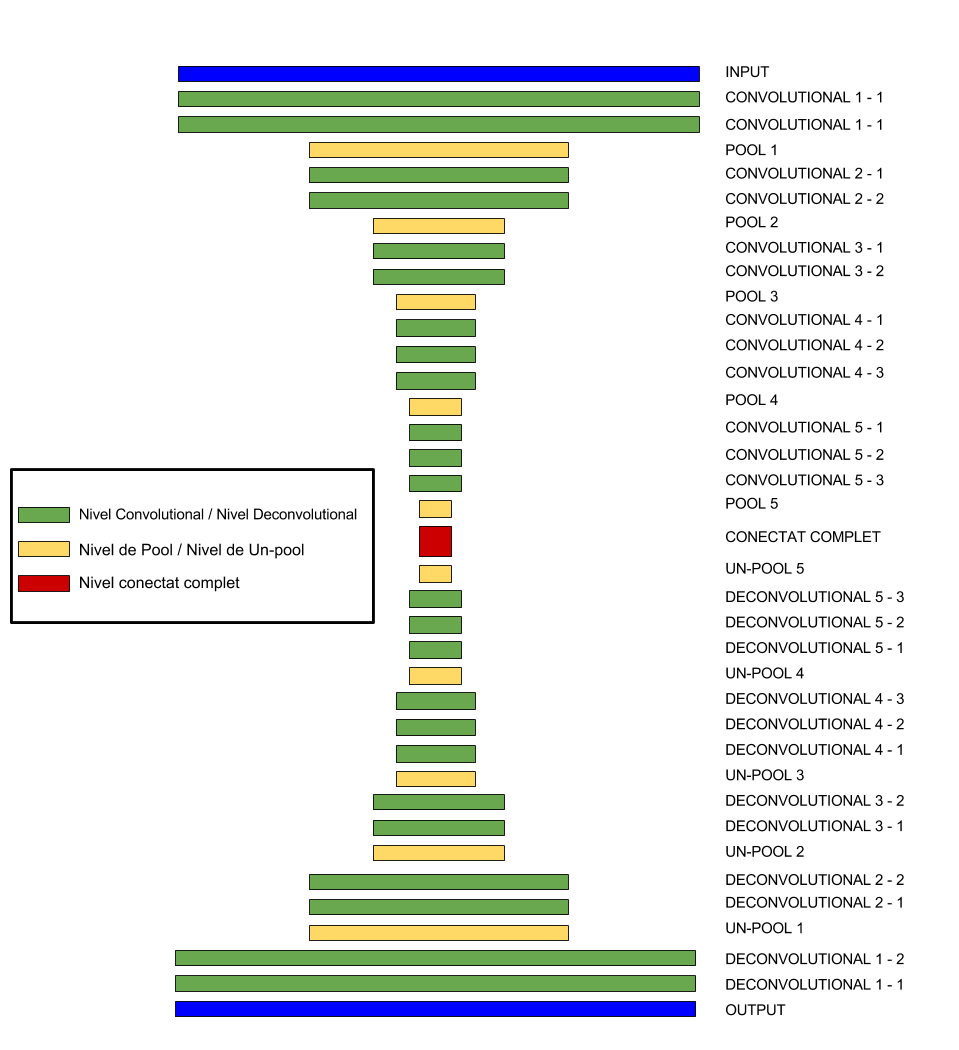
\includegraphics[width=500]{arhitectura_segmentor.png}
\end{center}

\^{I}n imaginea de mai sus am ilustrat nivelele din re\c{t}eaua neuronal\u{a}, unde am reprezentat prin culoarea verde nivelele convolu\c{t}ionale \c{s}i deconvolu\c{t}ionale, prin galben nivelele de pool \c{s}i de un-pool, iar prin ro\c{s}u nivelul conectat complet.

\par

Nivelele deconvolu\c{t}ionale \c{s}i nevelele de un-pool sunt nivele ce se comport\u{a} invers fa\c{t}\u{a} de nivelul convolu\c{t}ionl, respectiv nivelul de pool. Mai exact, nivelul de un-pool m\u{a}re\c{s}te spa\c{t}iul dimensional pe baza pozi\c{t}iilor care au trecut de nivelul de pool, iar nivelul deconvolu\c{t}ional este de fapt transpusa nivelului convolu\c{t}ional.

\par

\^{I}n arhitectura ilustrat\u{a} mai sus, am pus dup\u{a} fiecare nivel convolu\c{t}ional c\^{a}te o func\c{t}ie de activare ReLU, iar nivelele convolu\c{t}ionale \c{s}i deconvolu\c{t}ionale au ponderi de dimensiune [3x3] cu un pas de glisare a ferestrei egal cu unu \^{i}n toate direc\c{t}iile de deplasere. Am ini\c{t}ializat ponderile de la nivelele convolu\c{t}ionale \c{s}i deconvolu\c{t}ionale cu variabile aleatoare dintr-o distribu\c{t}ie normal\u{a}, unde devia\c{t}ia standard este setat\u{a} la $\frac{1}{\sqrt{n}}$, unde n reprezint\u{a} numarul de variabile, iar bias-ul a fost setat la valoarea zero. Padding-ul a fost setat astfel \^{i}nc\^{a}t dimensiunea datelor de intrare, pe lungime \c{s}i \^{i}n\u{a}l\c{t}ime, s\u{a} se p\u{a}streze la datele rezultate \^{i}n urma aplic\u{a}rii nivelelor convolu\c{t}ionale \c{s}i deconvolu\c{t}ionale.

\par

Nivelul de pool \c{s}i un-pool, le-au fost setate o fereastr\u{a} de dimensiune [2x2] cu un pas de glisare a ferestrei egal cu doi, astfle \^{i}nc\^{a}t cantitatea de date s\u{a} se reduc\u{a} cu un procent de 75\% dup\u{a} aplicarea unui nivel de pool, respectiv s\u{a} se mareasc\u{a} cu un procent de 75\% dup\u{a} aplicarea unui nivel de un-pool.

\begin{center}
 \begin{longtable}{|p{4cm}|p{3cm}|p{3cm}|p{3cm}|} 
 \hline
 Nume & Dimensiune date de intrare & Numar ponderi \c{s}i bias-uri & Dimensiune date de ie\c{s}ire \\ [0.5ex] 
 \hline\hline
 Convolutional 1 - 1 &  [224 x 224 x 1] & 32 & [224 x 224 x 32] \\ 
 \hline
 Convolutional 1 - 2 & [224 x 224 x 32] & 32 & [224 x 224 x 32] \\
 \hline
 Pool 1 & [224 x 224 x 32] & - & [112 x 112 x 32] \\
 \hline
 Convolutional 2 - 1 & [112 x 112 x 32] & 64 & [112 x 112 x 64] \\
 \hline
 Convolutional 2 - 2 & [112 x 112 x 64] & 64 & [112 x 112 x 64] \\
 \hline
 Pool 2 & [112 x 112 x 64] & - & [56 x 56 x 64] \\
 \hline
 Convolutional 3 - 1 & [56 x 56 x 64] & 128 & [56 x 56 x 128] \\
 \hline
 Convolutional 3 - 2 & [56 x 56 x 128] & 128 & [56 x 56 x 128] \\
 \hline
 Pool 3 & [56 x 56 x 128] & - & [28 x 28 x 128] \\
 \hline
 Convolutional 4 - 1 & [28 x 28 x 128] & 256 & [28 x 28 x 256] \\
 \hline
 Convolutional 4 - 2 & [28 x 28 x 256] & 256 & [28 x 28 x 256] \\
 \hline
 Convolutional 4 - 3 & [28 x 28 x 256] & 256 & [28 x 28 x 256] \\
 \hline
 Pool 4 & [28 x 28 x 256] & - & [14 x 14 x 256] \\
 \hline
 Convolutional 5 - 1 & [14 x 14 x 256] & 256 & [14 x 14 x 256] \\
 \hline
 Convolutional 5 - 2 & [14 x 14 x 256] & 256 & [14 x 14 x 256] \\
 \hline
 Convolutional 5 - 3 & [14 x 14 x 256] & 256 & [14 x 14 x 256] \\
 \hline
 Pool 5 & [7 x 7 x 256] & - & [7 x 7 x 256] \\
 \hline
 Conectat complet & [7 x 7 x 256] & 4096 & [1 x 1 x 4096] \\
 \hline
 Deconectat complet & [1 x 1 x 4096] & 256 & [7 x 7 x 256] \\
 \hline
 Un-pool 5  & [7 x 7 x 256] & - & [14 x 14 x 256] \\
 \hline
 Deconvolutional 5 - 3 & [14 x 14 x 256] & 256 & [14 x 14 x 256] \\
 \hline
 Deconvolutional 5 - 2 & [14 x 14 x 256] & 256 & [14 x 14 x 256] \\
 \hline
 Deconvolutional 5 - 1 & [14 x 14 x 256] & 256 & [14 x 14 x 256] \\
 \hline
 Un-pool 4  & [14 x 14 x 256] & - & [28 x 28 x 256] \\
 \hline
 Deconvolutional 4 - 3 & [28 x 28 x 256] & 256 & [28 x 28 x 256] \\
 \hline
 Deconvolutional 4 - 2 & [28 x 28 x 256] & 256 & [28 x 28 x 256] \\
 \hline
 Deconvolutional 4 - 1 & [28 x 28 x 256] & 128 & [28 x 28 x 128] \\
 \hline
 Un-pool 3  & [28 x 28 x 128] & - & [56 x 56 x 128] \\
 \hline
 Deconvolutional 3 - 2 & [56 x 56 x 128] & 128 & [56 x 56 x 128] \\
 \hline
 Deconvolutional 4 - 1 & [56 x 56 x 128] & 64 & [56 x 56 x 64] \\
 \hline
 Un-pool 2  & [56 x 56 x 64] & - & [112 x 112 x 64] \\
 \hline
 Deconvolutional 2 - 2 & [112 x 112 x 64] & 64 & [112 x 112 x 64] \\
 \hline
 Deconvolutional 2 - 1 & [112 x 112 x 64] & 32 & [112 x 112 x 32] \\
 \hline
  Un-pool 1  & [112 x 112 x 32] & - & [224 x 224 x 32] \\
 \hline
 Deconvolutional 1 - 2 & [224 x 224 x 32] & 32 & [224 x 224 x 32] \\
 \hline
 Deconvolutional 1 - 1 & [224 x 224 x 32] & 32 & [224 x 224 x 32] \\
 \hline
 Output & [224 x 224 x 32] & 2 & [224 x 224 x 2] \\
 \hline
 Softmax & [224 x 224 x 2] & - & [224 x 224 x 2] \\
 \hline
 Argmax & [224 x 224 x 2] & - & [224 x 224 x 1] \\
 \hline
\end{longtable}
\end{center}

Cum am precizat \c{s}i mai sus, nivelele convolu\c{t}ionale \c{s}i deconvolu\c{t}ionale au ponderi de dimensiune [3 x 3], singurile nivele care nu respect\u{a} acest\u{a} dimensiune, sunt nivelele Conectat complet \c{s}i Deconectat complet, unde ponderile au o dimensiune de [7 x 7] pentru a conecta fiecare neuron cu fiecare ponder\u{a}. Alt nivel care nu respect\u{a} aceast\u{a} dimensiune este nivelul de Output, care are o dimensiune a ponderilor de [1 x 1], acest nivel are rolul de a aduce dimensiunea datelor, de la penultimul nivel deconvolu\c{t}ional, de la valoarea 32 la numarul de clase posbile, \^{i}n cazul nostru sunt doua clase posibile, exist\u{a} sau nu la pozi\c{t}ia respectiv\u{a} ventirculul st\^{a}ng a inimii, aceste clase sunt reprezentate prin valoarea 1 pentru posibilitatea c\u{a} exist\u{a} \c{s}i 0 pentru posibilitatea c\u{a} nu exist\u{a}.

\par

Dup\u{a} nivelul de Output se aplic\u{a} func\c{t}ia Softmax, ca func\c{t}ie de cost, pentru calcularea pierderii, iar pentru aflarea rezultatului final se aplic\u{a} o func\c{t}ie numit\u{a} Argmax, care \^{i}ntoarce pozi\c{t}ia unde valoarea este cea mai mare, aceast\u{a} func\c{t}ie este aplicat\u{a} pe ad\^{a}ncimea setului de date. Ceea ce \^{i}ntoarce func\c{t}ia Argmax reprezint\u{a} prezicerile pe care re\c{t}eaua neuronal\u{a} o face \^{i}n urma procesului de antrenare.

\par

\^{I}nainte ca setul de date de la spitalul Sunnybrook s\u{a} fie introduce \^{i}n re\c{t}eaua neuronal\u{a}, \^{i}n procesul de antrenare sau pentru preziceri, acestea trebuiesc mai \^{i}nt\^{a}i decupate astfel \^{i}nc\^{a}t s\u{a} intre \^{i}n re\c{t}eaua neuronal\u{a}. Cum se observ\u{a} \c{s}i \^{i}n tabelul de mai sus, re\c{t}eaua neuronal\u{a} accept\u{a} un set de date de dimensiunea [224 x 224], \^{i}ns\u{a} setul de date de la Sunnybrook are o dimensiune de [254 x 256]. Acest lucur a fost f\u{a}cut pentru a multimplica setul de date, din cauz\u{a} c\u{a} setul de date pus la dispozi\c{t}ie de spitalul Sunnybrook este destul de mic ( doar 805 de exemple ), trebuia s\u{a} gasim o modalitate de al multiplica, iar cea mai bun\u{a} solu\c{t}ie pe care am gasito pentru a face acest lucru a fost s\u{a} punem re\c{t}eaua neuronal\u{a} s\u{a} accepte un volum de date de dimensiune mai mic\u{a}, astfel \^{i}nc\^{a}t s\u{a} putem sa decup\u{a}m la o pozi\c{t}ie aleatoare setul de date. Prin urmare, \^{i}nainte s\u{a} introducem setul de date \^{i}n re\c{t}eaua neuronal\u{a}, alegem dou\u{a} valori aleatorii, una pentru axa Ox, alta pentru axa Oy, \c{s}i incepem s\u{a} decup\u{a}m de la acea pozi\c{t}ie, dup\u{a} aceea setul de date  decupat este centrat la zero \c{s}i normalizat, setul de date rezultat este introdus \^{i}n re\c{t}eaua neuronalu\u{a}.

\par

La procesul de antrenare,  am ales metoda Adam pentru antrenare, rata de \^{i}nv\u{a}\c{t}are a fost setat\u{a} la valoarea de 1e-6, \c{s}i s-au efectuat 40 de itera\c{t}ii peste setul de date, iar la fiecare pas de antrenare s-au luat c\^{a}te doua exemple din setul de date. Din cele 805 de exemple de antrenare, puse la dispozi\c{t}ie de spitalul Sunnybrook, am p\u{a}strat 5 valori pentru a vedea ce preziceri face re\c{t}eaua neuronal\u{a} peste date pe care nu le-a vazut niciodat\u{a} \^{i}n procesul de antrenare, celelate 800 de exemple au fost folosite \^{i}n procesul de antrenare. Cu 800 de exemple de antrenare, din care s-au luat 2 exemple la fiecare pas de antrenare, la fiecare pas de itera\c{t}ie peste setul de date s-au efectuat 400 de pa\c{s}i de antrenare, av\^{a}nd \^{i}n vedere c\u{a} s-au f\u{a}cut 40 de itera\c{t}ii peste setul de dat avem un total de 160.000 de pa\c{s}i de antrenare. L-a fiecare itera\c{t}ie peste setul de date ( numit si epoch ) s-au salvat parametrii re\c{t}elei neuronale \c{s}i s-a calculat func\c{t}ia total\u{a} de cost peste setul de date.

\begin{center}
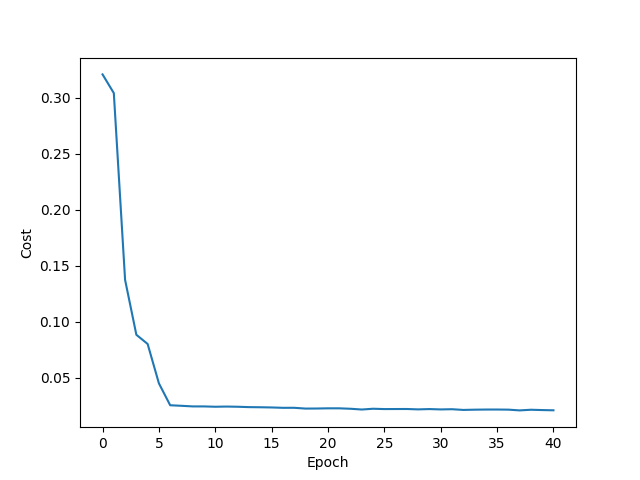
\includegraphics[width=400]{loss.png}
\end{center}

\^{I}n graficul de mai sus s-a ilustrat progresul func\c{t}iei de cost la fiecare epoch, ce-a mai mic\u{a} valoare a fost atins\u{a} la epoch-ul 40, unde func\c{t}ia de cost a ar\u{a}tat o valoare de 0.019257. Procesul de antrenare a durat 5 ore pe un nvidia geforce titan x, iar re\c{t}eaua neuronal\u{a} a fost scris\u{a} in Python 3.5 cu ajutorul libr\u{a}riei TensorFlow.

\^{I}n imaginile de mai jos pute\c{t}i vedea prezicerile pe care re\c{t}eaua neuronal\u{a} le-a f\u{a}cut pe seteul de date care nu a fost inclus \^{i}n procesul de antrenare ( cele 5 exemple ). Motivul pentru care se exclud unele date din procesul de antrenare pentru a se face preziceri pe ele este acela de a vedea cum se descurc\u{a} re\c{t}eaua neuronal\u{a} pe un set de date pe care nu l-a vazut niciodat\u{a} \c{s}i pentru a ne asigura c\u{a} re\c{t}eaua neuronal\u{a} nu a \^{i}nv\u{a}\c{t}at pe dinafar\u{a} datele de antrenare ( efectul de overfitting ).

\par

Setul de imagine pe care le vom prezenta, \^{i}n cele ce urmeaz\u{a}, sunt structurate pe dou\u{a} coloane, pe prima coloan\u{a} sunt raspunsurile, pe care re\c{t}eaua neuronal\u{a} ar trebuii s\u{a} le prezic\u{a}, iar pe a do\u{a} coloan\u{a} sunt prezicerile pe care le-a facut re\c{t}eaua neuronal\u{a}. Pe fiecare coloana exist\u{a} trei randuri de imagini, unde pe primul r\^{a}nd este imagine pe care se face prezicerea, pe al doilea r\^{a}nd este prezicerea f\u{a}cut\u{a}, iar pe r\^{a}ndul trei este imaginea decupat\u{a} de pe primul r\^{a}nd pe baza prezicerilor de pe r\^{a}ndul doi.

\begin{center}
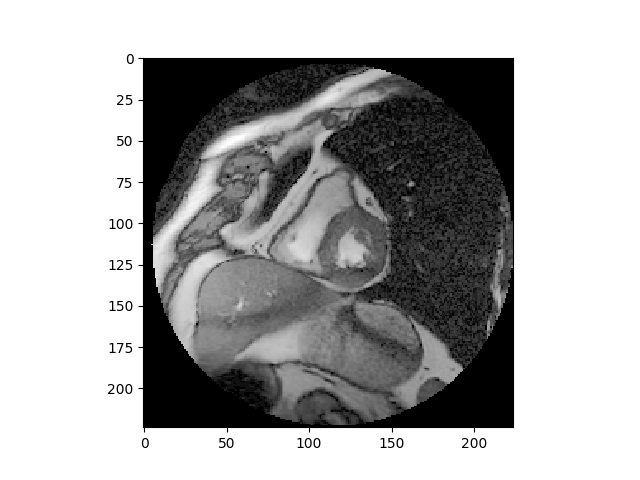
\includegraphics[width=200]{1_image.png}
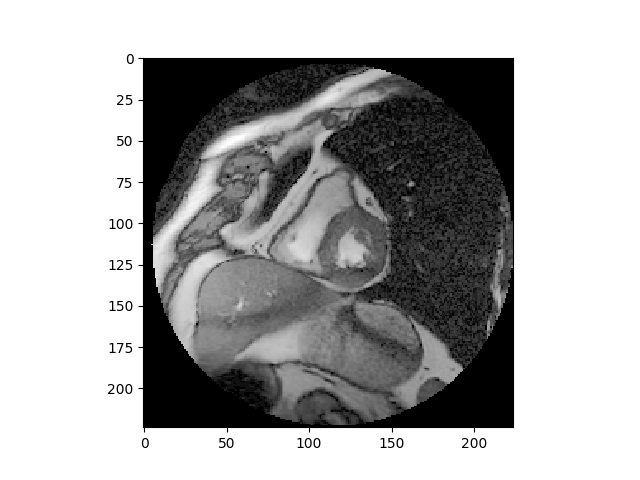
\includegraphics[width=200]{1_image.png}
\end{center}

\begin{center}
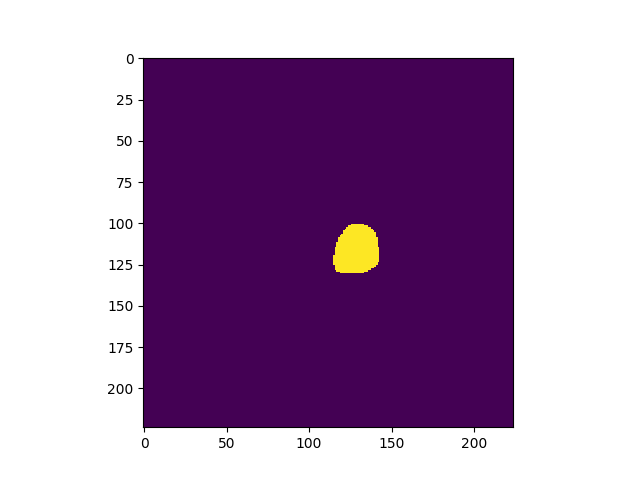
\includegraphics[width=200]{1_labels.png}
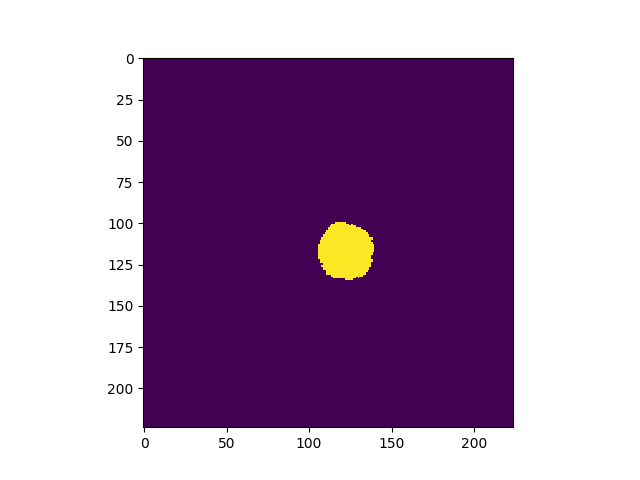
\includegraphics[width=200]{1_labels_predict.png}
\end{center}

\begin{center}
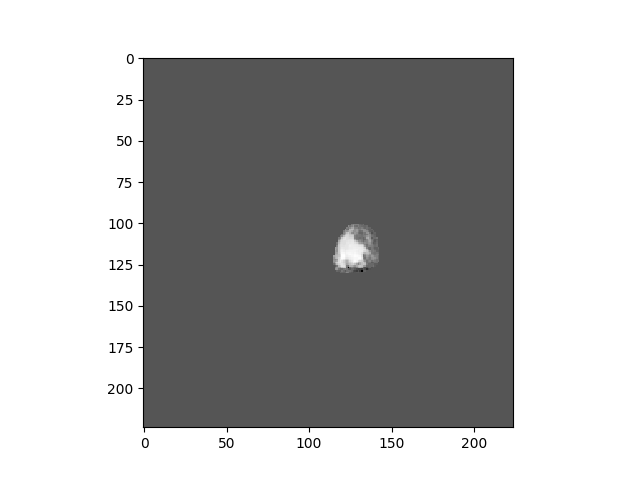
\includegraphics[width=200]{1_image_labels.png}
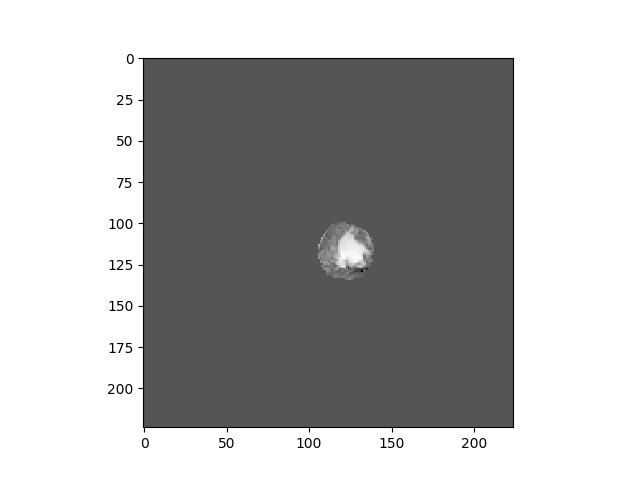
\includegraphics[width=200]{1_image_predict.png}
\end{center}

\^{I}n imaginile de mai sus, pe partea dtreapt\u{a}, sunt ilustrate rezultatele ob\c{t}inute la prezicere la primul exemplu, iar pe partea st\^{a}ng\u{a} este adev\u{a}rata valoare. Se poate observa faltul c\u{a}, prezicerea f\u{a}cut\u{a} de re\c{t}eaua neuronal\u{a} este destul de aproape de adev\u{a}r ( r\^{a}ndurile doi \c{s}i trei ), \^{i}ns\u{a} exist\u{a} diferen\c{t}e \^{i}ntre ele, cum ar fi spre exemplu faptul c\u{a} rec\c{t}eaua neuronal\u{a} a prezis ventriculul st\^{a}ng ceva mai la st\^{a}nga \c{s}i pu\c{t}in mai mare dec\^{a} era cu adev\u{a}rat.

\begin{center}
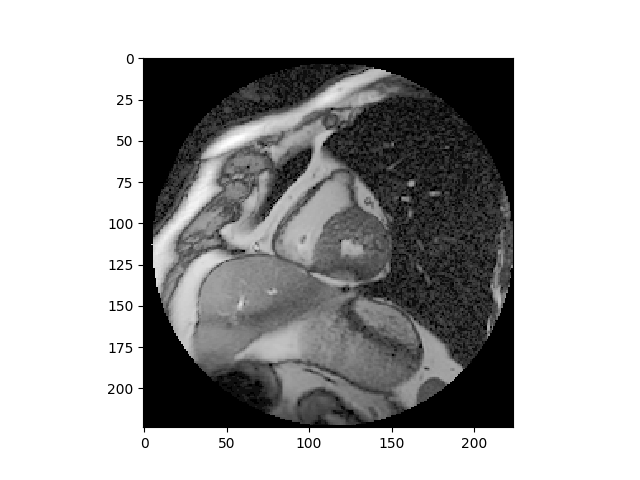
\includegraphics[width=200]{2_image.png}
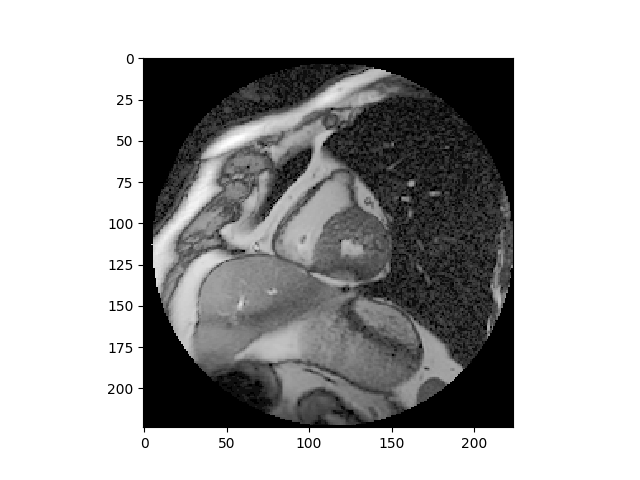
\includegraphics[width=200]{2_image.png}
\end{center}

\begin{center}
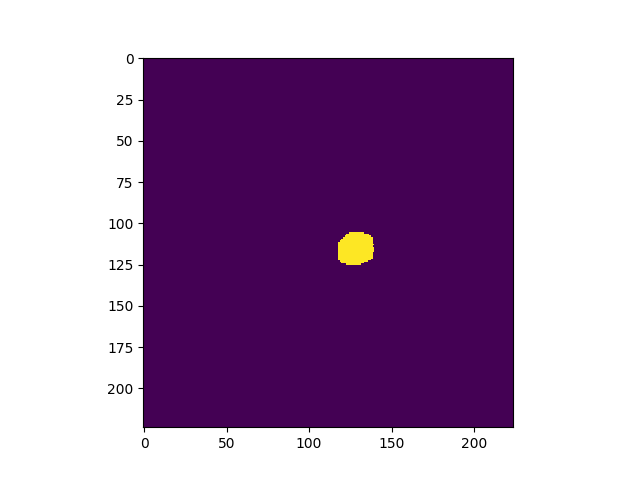
\includegraphics[width=200]{2_labels.png}
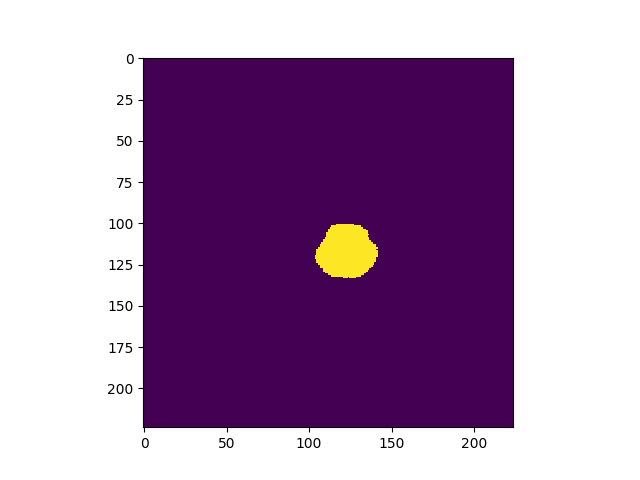
\includegraphics[width=200]{2_labels_predict.png}
\end{center}

\begin{center}
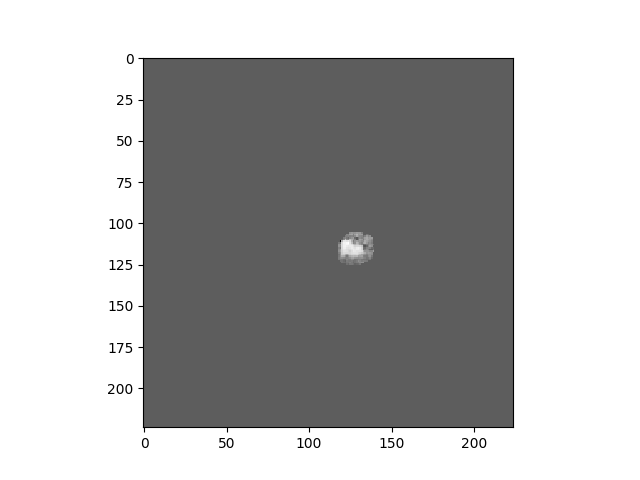
\includegraphics[width=200]{2_image_labels.png}
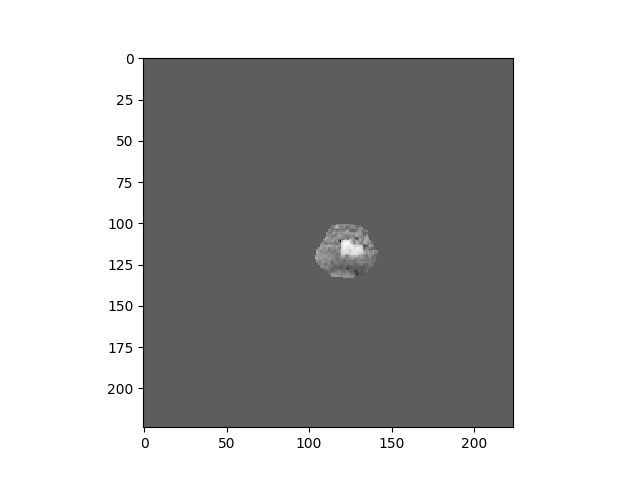
\includegraphics[width=200]{2_image_predict.png}
\end{center}

Prezicerea pe imaginea doi este ilustrat\u{a} mai sus. Se poate vedea c\u{a} rec\c{t}eaua neuronal\u{a} de data asta a prezis un ventricul st\^{a}ng mult mai mare de data asta dec\^{a}t era cu adev\u{a}rat. Acest lucru s-ar putea datora faptului c\u{a}, pe setul de imagini de antrenare, erau mai multe imagini cu ventriculul st\^{a}ng c\^{a}nd era la diastol\u{a} dec\^{a}t cele care erau la sistol\u{a}, iar din aceast\u{a} cauz\u{a} re\c{t}eaua neuronal\u{a} a prezis un ventricul st\^{a}ng a\c{s}a de mare, pentru c\u{a} a \^{i}nv\u{a}\c{t}at s\u{a} caute ventricule aflate la diastol\u{a}.

\begin{center}
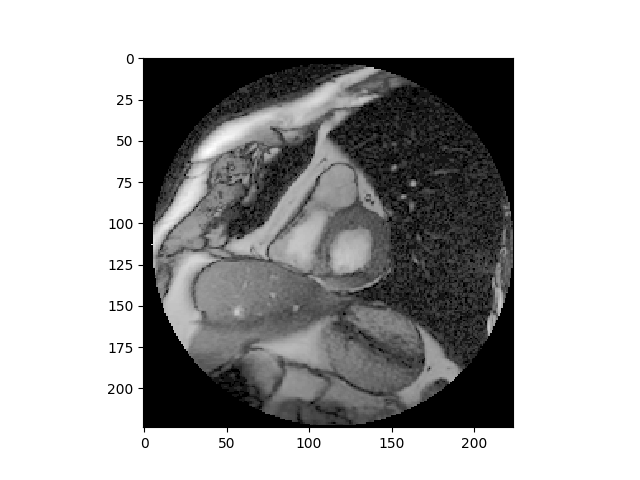
\includegraphics[width=200]{3_image.png}
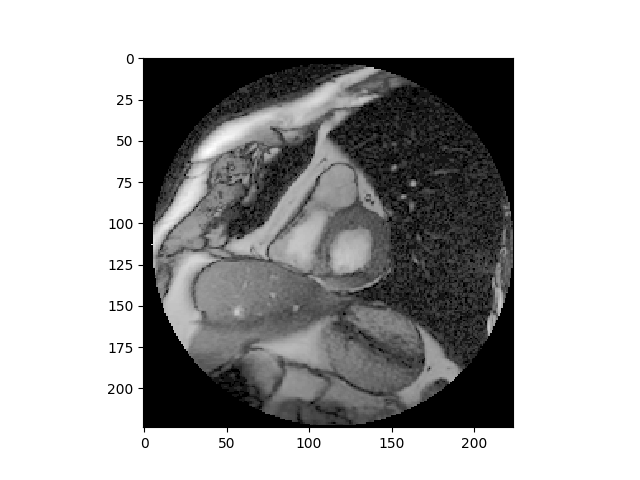
\includegraphics[width=200]{3_image.png}
\end{center}

\begin{center}
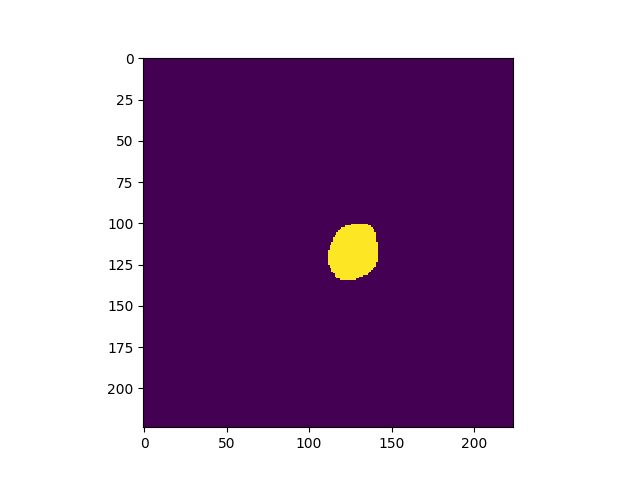
\includegraphics[width=200]{3_labels.png}
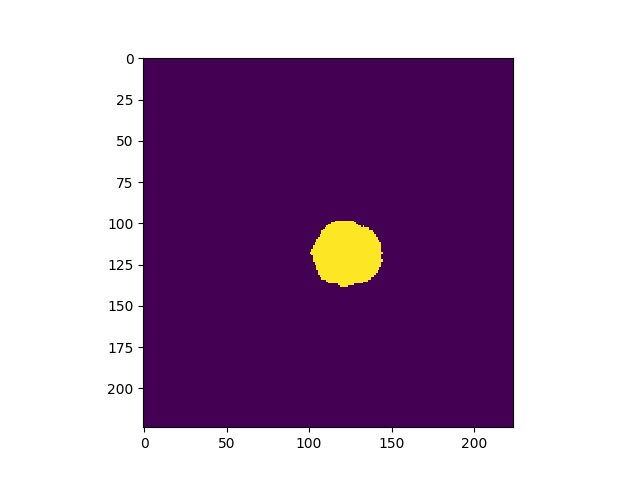
\includegraphics[width=200]{3_labels_predict.png}
\end{center}

\begin{center}
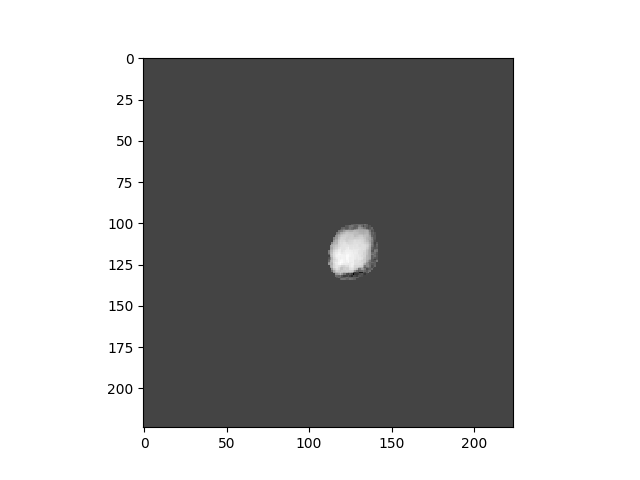
\includegraphics[width=200]{3_image_labels.png}
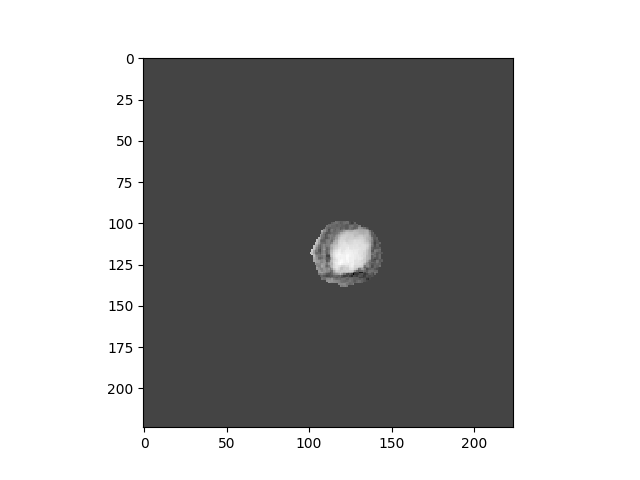
\includegraphics[width=200]{3_image_predict.png}
\end{center}

Pe setul de imagini trei, pe care s-a facut prezicerea de c\u{a}tre rec\c{t}eauan neuronal\u{a}, avem aceea\c{s}i problem\u{a}, re\c{t}eaua neuronal\u{a} face preziceri mult mari a ventricului st\^{a}ng dec\^{a}t sunt ele de fapt \^{i}n realitate. De data aceasta \^{i}ns\u{a} se poate trece cu vederea acest fapt, deoarece inima acum se afl\u{a} la diastol\u{a}, iar ventriculul st\^{a}ng este la expansiunea sa maxim\u{a}, iar prezicerea, dup\u{a} cum se poate observa, sunt destul de aproape de adev\u{a}r.

\begin{center}
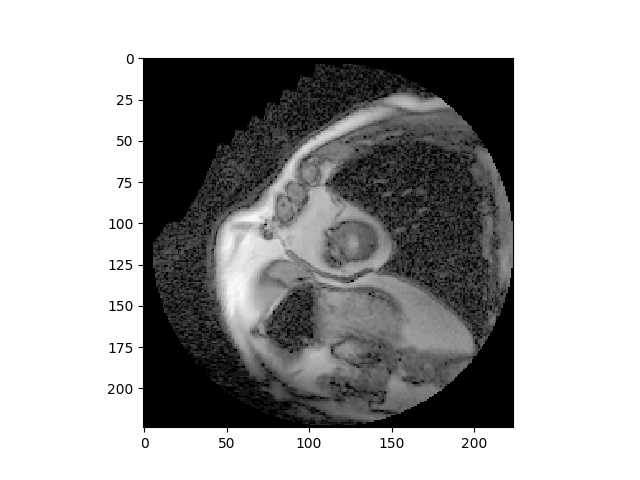
\includegraphics[width=200]{4_image.png}
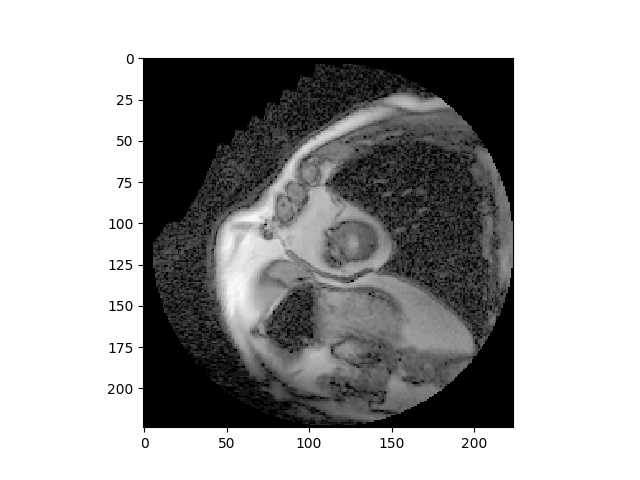
\includegraphics[width=200]{4_image.png}
\end{center}

\begin{center}
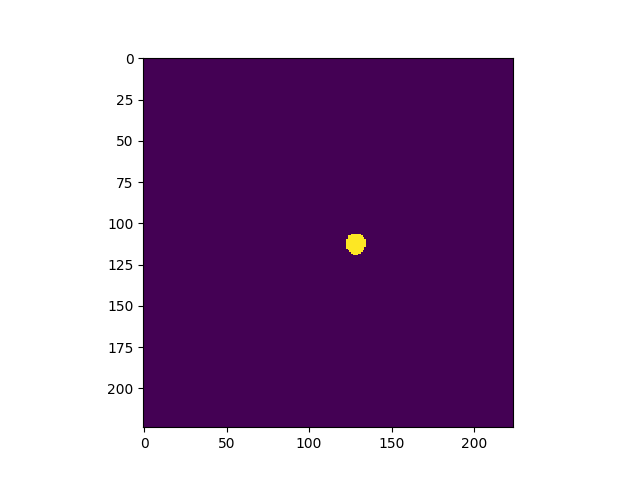
\includegraphics[width=200]{4_labels.png}
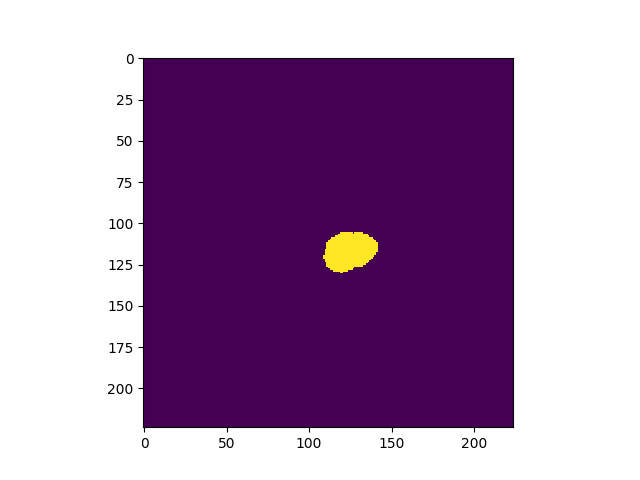
\includegraphics[width=200]{4_labels_predict.png}
\end{center}

\begin{center}
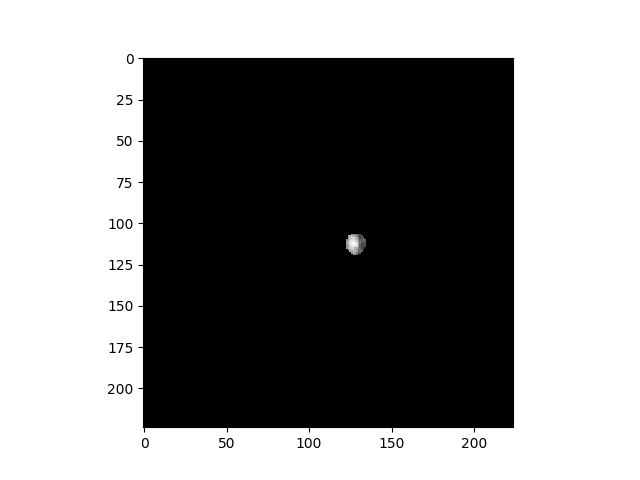
\includegraphics[width=200]{4_image_labels.png}
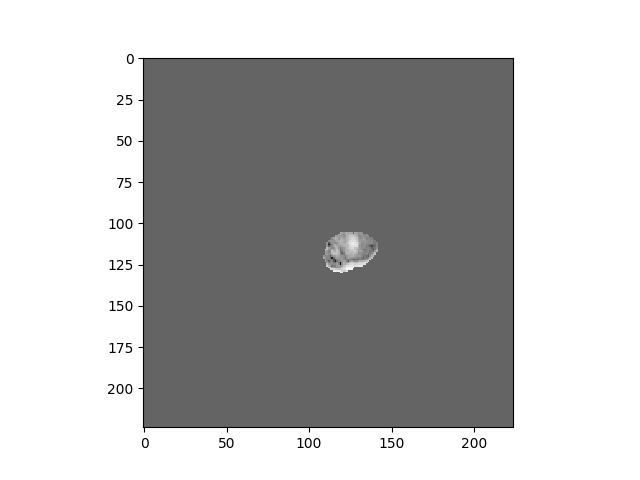
\includegraphics[width=200]{4_image_predict.png}
\end{center}

Penultimul set de date pe care s-a f\u{a}cut prezicerea este cel mai interesant, deoarece inima se afl\u{a} la sistol\u{a}, iar ventriculul st\^{a}ng este greu de detectat \c{s}i cu ochiul liber, \^{i}ns\u{a} re\c{t}eaua neuronal\u{a} a reu\c{s}it s\u{a} \^{i}l detecteze, ins\u{a} a facut iar aceea\c{s}i gre\c{s}teal\u{a} ca \c{s}i la celelalte cazuri, a dectectat un ventricul st\^{a}ng mult mai mare dec\^{a}t este el de fapt. Dup\u{a} cum se poate observa, ventriculul st\^{a}ng detectat acum de re\c{t}eaua neuronal\u{a} este de vreo cinci ori mai mare dec\^{a}t ar trebuii s\u{a} fie, acest lucru fiind pus pe seama faptului c\u{a}, \^{i}n setul de date de antrenare exist\u{a} pu\c{t}ine exeple cu un ventricul st\^{a}ng a\c{s}a de mic.

\begin{center}
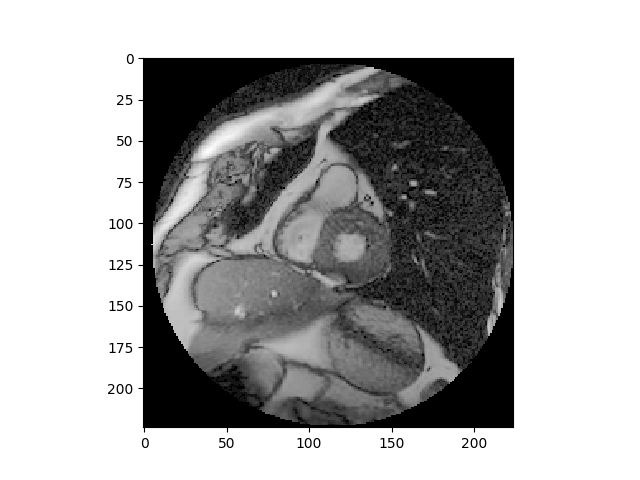
\includegraphics[width=200]{5_image.png}
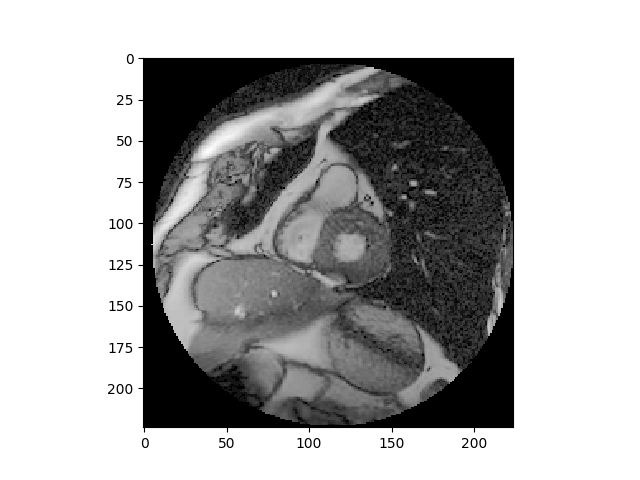
\includegraphics[width=200]{5_image.png}
\end{center}

\begin{center}
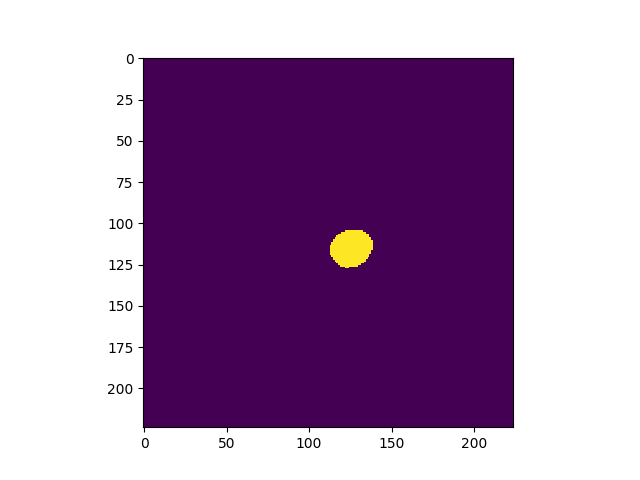
\includegraphics[width=200]{5_labels.png}
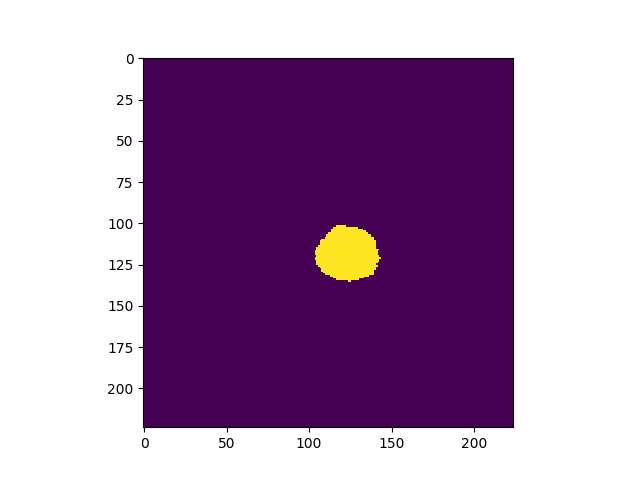
\includegraphics[width=200]{5_labels_true.png}
\end{center}

\begin{center}
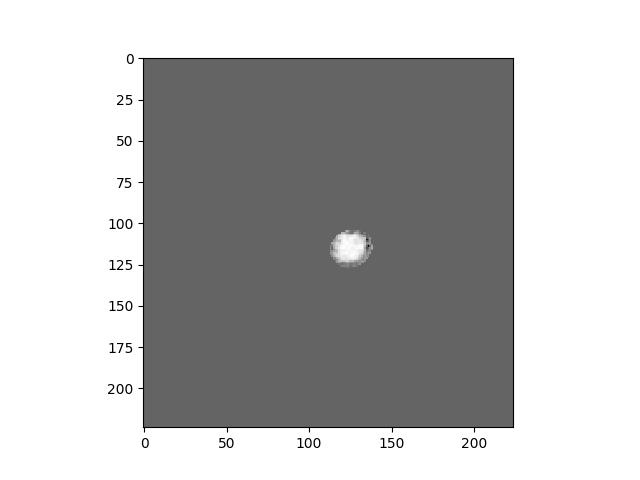
\includegraphics[width=200]{5_image_labels.png}
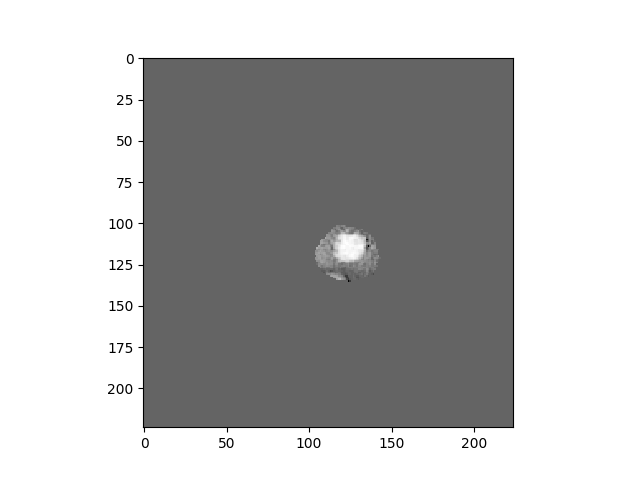
\includegraphics[width=200]{5_image_predict.png}
\end{center}

Pe ultimul set de date pe care s-a f\u{a}cut prezicerea se poate observa c\u{a} exist\u{a} aceea\c{s}i problem\u{a}, un ventricul st\^{a}ng mult mai mare detectat.

\par

Din imaginile ilustrate mai sus putem s\u{a} tragem o concluzie, aceea c\u{a}, re\c{t}eaua neuronal\u{a} face detec\c{t}ii a ventricului st\^{a}ng mult prea mari, \^{i}ns\u{a} sunt acceptabile pentru a trece la urm\u{a}torul pas, acela de a prezice volumul de s\^{a}nge care curge prin ventriculul st\^{a}ng. O posibil\u{a} modalitate de a for\c{t}a re\c{t}eaua neuronal\u{a} s\u{a} prezic\u{a} un ventricul st\^{a}ng mai mic ar fi s\u{a} supliment\u{a}m num\u{a}rul de imagine de antrenare cu inimi aflate la sistol\u{a}.

\section{Prezicerea volumului de s\^{a}nge}

Dup\u{a} antrenarea re\c{t}eleu neuronale pentru a segmenta ventriculul st\^{a}ng a inimii, putem trece la pasul de a prezice volumul de s\^{a}nge care curge prin inim\u{a}.

\par

Primul pas \^{i}n realizarea acestui lucru este de a citi datele salvate din fi\c{s}ierul CSV, date pe care le-am salvat din metadatele de la fi\c{s}ierele DICOM aferent fiecarui pacient. Dup\u{a} citim fiecare imagine PNG care provine de la un pacient, \^{i}ns\u{a} din cauza faptului c\u{a} fiecare imagine are o dimensiune de [256 x 256] iar re\c{t}eaua neuronal\u{a} care face segmentarea ventricului st\^{a}ng accept\u{a} doar imagine de dimensiunea [224 x 224] vom fi nevoi\c{t}i s\u{a} mai t\u{a}iem din fiecare imagine c\^{a}te 32 de pixeli pe orizontal\u{a} \c{s}i vertical\u{a} ca s\u{a} \^{i}i aducem la dimensiunea corespunz\u{a}toare.

\par

Al doilea pas \^{i}l presupune trecerea imaginilor, ale unui pacient, prin re\c{t}eaua neuronal\u{a}, pentru a se segmenta ventriculul st\^{a}ng al inimii. \^{I}nainte de a introduce imaginile \^{i}n re\c{t}eaua neuronal\u{a}, acestea trebuiesc normalizate \c{s}i centrate la zero. Dup\u{a} introducerea imaginilor \^{i}n re\c{t}eaua neuronal\u{a} \c{s}i ob\c{t}inerea rezultatelor, acestea sunt salvate sub format PNG \^{i}ntr-un fi\c{s}ier.

\par

Al treilea pas \^{i}l presupune num\u{a}rarea pixelilor care fac parte din ventriculul st\^{a}ng al inimii \c{s}i salvarea acestor valori pentru pa\c{s}ii urm\u{a}tori.

\par 

Al patrulea pas, \c{s}i ultimul din aceast\u{a} faz\u{a}, este calcularea efectiva a cantit\u{a}\c{t}ii de s\^{a}nge care curge prin ventriculul st\^{a}ng la momentul respectiv. Prima dat\u{a} se va stabilii care frame apar\c{t}ine sistolei \c{s}i care apar\c{t}ine diastolei, aces lucur se va face cu ajutorul numarului de pixeli detecteta\c{t}i de re\c{t}eaua neuronal\u{a}, astfel \^{i}nc\^{a}t frame-ul cu cei mai pu\c{t}ini pixeli va fi atribuit  sistolei, iar frame-ul cu cei mai mul\c{t}i pixeli va fi atribuit diastolei. Dup\u{a} determinarea frame-urilor care apar\c{t}ine siastolei si diastolei se poate calcula volumul de s\^{a}nge la siastol\u{a} \c{s}i la diastol\u{a}. Se iau toate pozele care apar\c{t}in respectivelor frame-uri iar numarul de pixeli pe care \^{i}l au se \^{i}nmul\c{t}este cu distan\c{t}a dintre ele, iar rezultatul ob\c{t}inut reprezint\u{a} volumul de s\^{a}nge care curge la diastol\u{a}, respectiv sistol\u{a}, \^{i}n fram-ul respectiv. Pentru a calcula volumul total care curge \^{i}n toate fram-urile vom proceda \^{i}n felul urm\u{a}tor, vom lua pentru fiecare frame ( \^{i}l vom nota cu $f$ ) fram-ul din fa\c{t}a lui (\^{i}l vom nota cu $f_v$ ) \c{s}i distan\c{t}a dintre ele (\^{i}l vom nota cu $\Delta$ ) \c{s}i vom aplica urm\u{a}toare formul\u{a}:

$$ V = \frac{1}{1000} \sum_i \Delta_i \frac{f_i + \sqrt{f_i * f_{v_i}} + f_{v_i}}{3} $$

Valoarea 1000 care apare \^{i}n fa\c{t}a formulei este un parametru pus din cauz\u{a} c\u{a} de cele mai multe ori calculul volumului de s\^{a}nge ie\c{s}ea de cele mai multe ori mult prea mare de c\^{a}t ar fi trebuit, din aceast\u{a} cauz\u{a} a fost ad\u{a}ugat \^{i}n formul\u{a}.

\par

Rezultatele ob\c{t}inute la pasul patru vor fi salvate intr-un fi\c{s}ier CSV. De precizat faptul c\u{a} acestea nu sunt valorile finale \c{s}i nu vom calcula la acest pas frac\c{t}ia de ejec\c{t}ie a inimii deoarece, a\c{s}a cum am vazut \c{s}i \^{i}n capitolul anterior, re\c{t}eaua noastr\u{a} neuronal\u{a} nu face preziceri tocmai perfect \c{s}i din acest\u{a} cauz\u{a} vom mai face o calibrare a datelor calculate, astfel \^{i}nc\^{a}t acestea s\u{a} fiu c\^{a}t mai aproape de adev\u{a}r.

\section{Calibrarea datelor}

Pentru a face partea de calibrare a datelor prezise de re\c{t}eaua neuronal\u{a} pentru volum de s\^{a}nge care curge la sistol\u{a} \c{s}i diastol\u{a} ne vom folosii de restul datelor pe care le oferea fi\c{s}ierele DICOM (num\u{a}rul de linii, numarul de coloane pe care le are o radiografie, spa\c{t}iul dintre frame-uri, grosimea radiografiei, v\^{a}rsta pacientului, unghiul din care a fost f\u{a}cut\u{a} radiografia) pe l\^{a}ng\u{a} acestea vom mai ad\u{a}uga \c{s}i valorile calculate pe baza prezicerilor f\u{a}cute de re\c{t}eaua neuronal\u{a} pentru sistol\u{a} \c{s}i diastol\u{a}. Cu ajutorul acestor date vom folosii algoritmul \textbf{\textit{Gradient Bootstrap}} pentru a prezice diferen\c{t}a dintre valorile reale la sistol\u{a} \c{s}i diastol\u{a} \c{s}i valorile prezise.

\par

Pentru algoritmul \textbf{\textit{Gradient Bootstrap}} vom folosii ca date de antrenare pacien\c{t}ii pentru care \c{s}tiim valorile adev\u{a}rate la sistol\u{a} \c{s}i diastol\u{a} ( sunt 700 de pacienti din 1140 pentru care s\c{t}iim valorile reale la sistol\u{a} \c{s}i diastol\u{a} ) iar pentru ceilal\c{t}i pacien\c{t}i vom prezice aceste dou\u{a} valori.

\par

\textbf{\textit{Gradient Bootstrap}} este un algoritm de Machine Learning folosit pentru probleme de regresii \c{s}i clasificare. Acesta se folose\c{s}te de un arbore de decizii pe care \^{i}l construie\c{s}te ca s\u{a} minimizeze funnc\c{t}ia de pierdere, unde func\c{t}ia de pierdere reprezint\u{a} diferen\c{t}a la p\u{a}trat dintre prezicerea f\u{a}cut\u{a} \c{s}i prezicerea f\u{a}cut\u{a} de c\u{a}tre algoritm.

$$ f = (y - y_p )^2 $$

Fiecare prezicerea nou\u{a} este f\u{a}cut\u{a} pe baza prezicerilor anterioare, astfle \^{i}nc\^{a}t fiecare nou nivel este consturit ca s\u{a} minimizeze func\c{t}ia de cost al nivelului anterior.

\begin{center}
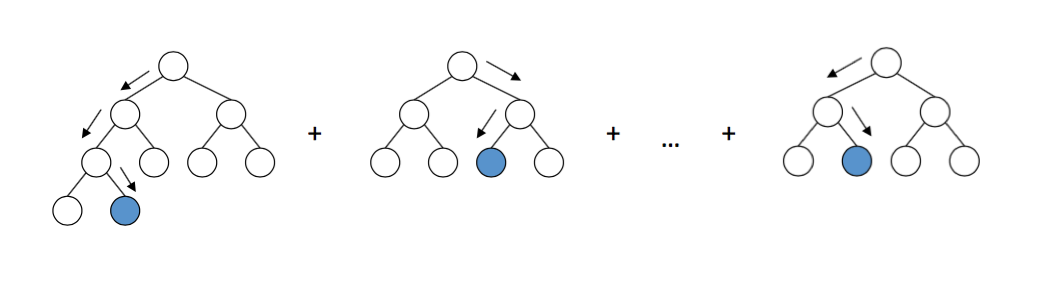
\includegraphics[width=400]{gradinet_boosting.png}
\end{center} 

Pentru algoritmul \textbf{\textit{Gradient Bootstrap}} am ales urm\u{a}torii parametrii pentru a se efectua partea de regresie \^{i}n prezicerea diferen\c{t}elor dintre sistol\u{a}, respectiv diastol\u{a}, a valorilor reale cu valorile calculate la pacien\c{t}ii pentru care nu \c{s}tiim valorile reale la sistol\u{a} \c{s}i diastol\u{a}. Ca rat\u{a} de \^{i}nv\u{a}\c{t}are am ajuns \^{i}n urma experimentelor la valoarea 0.001, acesta fiind \c{s}i cel mai greu parametru de setat. Ca num\u{a}r maxim de nivele am l\u{a}sat valorea 3, aceast\u{a} valoarea a fost aleas\u{a} pentru a prevenii efectul de overfitting, iar numarul minim de frunze la un nod a fost lasat la valoarea 2, iar num\u{a}rul maxim de estimatori a fost setat la 2500, tot din motivul de a se prevenii efectul de overfitting.

\par

Dup\u{a} aflarea valorilor prezise de c\u{a}tre algoritm putem calcula noile preziceri pentru sistol\u{a} \c{s}i diastol\u{a}, acestea vor reprezenta diferen\c{t}a dintre valorea calculat\u{a} pe baza prezicerilor f\u{a}cute de c\u{a}tre re\c{t}eaua neuronal\u{a} \c{s}i eroarea dintre valoarea prezis\u{a} \c{s}i valoarea adev\u{a}rat\u{a} pe care algoritmul \^{i}l indic\u{a}. 

\par

Valorile rezultate \^{i}n urma calculelor de mai sus reprezint\u{a} valorile finale pentru cantitatea de s\^{a}nge care curge la sistol\u{a} \c{s}i la diastol\u{a}, prin urmare acum se poate calcula frac\c{t}ia de ejec\c{t}ie, pe care o vom definii \^{i}n felul urm\u{a}tor:

$$ E_j = 100 * \frac{V_D - V_S}{V_D} $$

Unde $V_D$ reprezint\u{a} volumul de s\^{a}nge care curge la diastol\u{a}, iar $V_S$ reprezint\u{a} volumul de s\^{a}nge care curge la sistol\u{a} iar rezultatul final este reprezentat \^{i}n procent cu valori \^{i}ntre 0 \c{s}i 100. \^{I}n urma valorii rezultate se poate determina dac\u{a} un pacient are probleme cu inima \c{s}i c\^{a}t de grav este aceast\u{a} sau dac\u{a} este s\u{a}n\u{a}tos. Astfel c\u{a}, dac\u{a} frac\c{t}ia de ejec\c{t}ie este mai mare de 75\% atunci pacientul este declarat bolnav \c{s}i este hiperdinamic, dac\u{a} este \^{i}ntre 55\% \c{s}i 75\% atunci pacientul este declarat s\u{a}n\u{a}tos, dac\u{a} este 45\% \c{s}i 54\% atunci pacientul este declarat bolnav av\^{a}nd o frac\c{t}ie de ejec\c{t}ie u\c{s}or anormal\u{a}, dac\u{a} este \^{i}ntre 35\% \c{s}i 44\% atunci pacientul este delcarat bolnav cu o frac\c{t}ie de ejec\c{t}ie moderat anormal\u{a}, iar daca este sub 35\% atunci pacientul este bolnav cu o frac\c{t}ie de ejec\c{t}ie sever anormal\u{a}.

\section{Rezultate}

\^{I}n tabelul de mai jos sun prezentate c\^{a}teva example de rezultate ob\c{t}inute la pacien\c{t}ii pentru care nu se \c{s}tiau valorile reale a sistolei \c{s}i diastolei de la \^{i}nceput, de asemenea sunt ar\u{a}tate \c{s}i valorile lor reale pentru a putea fi comparate cu rezultatele ob\c{t}inute \c{s}i sunt calculate frac\c{t}iile de ejec\c{t}ie pentru valorile prezise \c{s}i valorile reale.

\begin{center}
 \begin{longtable}{|p{0.5cm}|p{2cm}|p{2cm}|p{2cm}|p{2cm}|p{2cm}|p{2cm}|} 
 \hline
 Nr. & Diastola real\u{a} & Diastola prezis\u{a} & Sistola real\u{a} & Sistola prezis\u{a} & Frac\c{t}ia de ejec\c{t}ie pentru valorile reale & Frac\c{t}ia de ejec\c{t}ie pentru valorile prezise  \\ [0.5ex] 
 \hline\hline
 1 &  158.0 & 158.7 & 76.0 & 63.61 & 51,8\% & 59,9\% \\
 \hline
 2 &  44.2 & 35.69 & 15.6 & 12.94 & 64,7\% & 63,7\% \\ 
 \hline
 3 &  129.7 & 128.44 & 83.2 & 38.6 & 35,8\% & 69,9\% \\
 \hline
 4 &  121.1 & 126.34 & 39.2 & 53.79 & 67,3\% & 57,4\% \\
 \hline
 5 &  127.4 & 145.78 & 57.8 & 57.99 & 54,63\% & 60,2\% \\
 \hline
 6 &  177.7 & 188.18 & 76.4 & 77.49 & 57\% & 58,8\% \\
 \hline
 7 &  277.6 & 186.16 & 133.5 & 74.88 & 51,9\% & 59,7\% \\
 \hline
 8 &  210.1 & 209.73 & 167.5 & 102.7 & 20,2\% & 51\% \\
 \hline
 9 &  230.1 & 193.51 & 91.4 & 91.53 & 60.2\% & 52,7\% \\
 \hline
 10 &  315.8 & 213.66 & 122.3 & 98.24 & 61,2\% & 54\% \\
 \hline
\end{longtable}
\end{center}

Dup\u{a} cum se poate vedea din tabelul de mai sus, metoda pe care am abordato \^{i}n acest\u{a} lucrare face unele preziceri destul de aproape de adev\u{a}r ( exemplele 2 \c{s}i 6) unde valorile diastolei \c{s}i sitolei prezie sunt destul de aproape de adev\u{a} astfel \^{i}nc\^{a}t ca frac\c{t}iile de ejec\c{t}ie s\u{a} ias\u{a} asem\u{a}n\u{a}toare. Mai sunt unele preziceri unde valorile diastolei sunt apropiate, \^{i}ns\u{a} din cauz\u{a} c\u{a} valorile sistolei difere \^{i}ntre ele, valorile frac\c{t}iei de ejec\c{t}ie ies la o diferen\c{t}\u{a} destul de mare \c{s}i din aceast\u{a} cauz\u{a} un pacient poate fi declarat bolnav sau s\u{a}n\u{a}tos din gre\c{s}eal\u{a} (exemplele 1, 3, 4 \c{s}i 8) sau invers, valorile sistoli s\u{a} fiu apropiate iar valorile diastolei s\u{a} au o diferen\c{t}\u{a} destul de mare \^{i}ntre el \c{s}i din aceast\u{a} cauz\u{a} s\u{a} diagnostic\u{a}m un pacient ca find s\u{a}n\u{a}tos sau bolnav ( exemplele 5 \c{s}i 9) sau cazul cel mai neprielnic, c\^{a}nd \c{s}i valorile sitolei \c{s}i diastolei prezise difer\u{a} foarte mult de valorile adev\u{a}rate \c{s}i din aceast\u{a} cauza iesi o diferen\c{t}\u{a} destul de mare \^{i}ntre cele dou\u{a} frac\c{t}ii de ejec\c{t}ie.